% !Mode:: "TeX:UTF-8"
%\chapter{车联网技术的网络资源优化理论基础}
\chapter{基于博弈论的鲁棒干扰管理异构车载网络中的大规模空地一体化通信
异构车载网络}
\begin{comment}
\label{chap:figures}
插图主要涉及到:单个居中图形;两个并排图形;两个以上的并排或者堆叠的图形;图题;图形的引用;
\end{comment}
\section{引言}\label{section2-1}
作为智能交通系统(ITS)最有前途的解决方案,车联网(IoV)有望满足快速增长的需求,如交通效率、驾驶体验和事故处理。然而,
由于车辆密度和用户需求的快速增加,单小区网络的频谱效率较低\cite{TFL}。因此,异构车载网络的部署已成为一种趋势。

近年来,空地一体化作为提高无线通信质量的最可行的解决方案之一,引起了工业界和学术界的广泛关注。由于无人机具有部署灵活、远程操作和
中继能力,选择空中无人机来辅助地面网络\cite{ACO}。然而,当无人机加入异构场景时,空地综合通信网络将面临两大挑战。首先,
当使用信道复用模式来提高频谱效率时,多用户干扰是一个棘手的问题。有效和鲁棒的通信在很大程度上受到多用户干扰的影响,特别
是在不确定的信道环境中,因此实现有效的干扰管理是一个重大挑战\cite{CCO}。 其次,空地集成异构车辆网络(AGHVN)是分层的,
其中蜂窝用户(CUE)和车辆用户(VUE)分别充当领导者和追随者。然而,CUE和VUE是不同的利益相关者,他们为自己的利益而竞争,
平衡各方利益是一项挑战,使用博弈论的决策方法可以有效的构建CUE和VUE之间复杂利益关系 \cite{胡益恺智能车辆决策方法研究综述}。
因此,空地一体化异构车载网络的广泛部署仍然带来紧迫的挑战。
\begin{comment}
\subsection{NOMA技术的理论基础}\label{section2-1-1}
大多数情况下,需要插入的图形是单个的时候可以使用如下环境:

\subsection{CR技术的理论基础}\label{section2-1-2}
其中的参数“[width=$\backslash$textwidth]”指定图形的宽度0.6倍页宽。最后的效果如图\ref{ysulogo}所示。
\begin{figure}[hptb!]
 \centering\small
 
\includegraphics[width=0.6\textwidth]{ysulogo}
 \Figcaption{单个居中图形}\label{ysulogo}
\end{figure}
\subsection{MEC技术的理论基础}\label{section2-1-3}

最终结果如图\ref{fig-dbfig}所示。
\begin{figure}[hptb!]
  \centering\small
  \begin{minipage}[t]{0.5\linewidth}
    \centering
    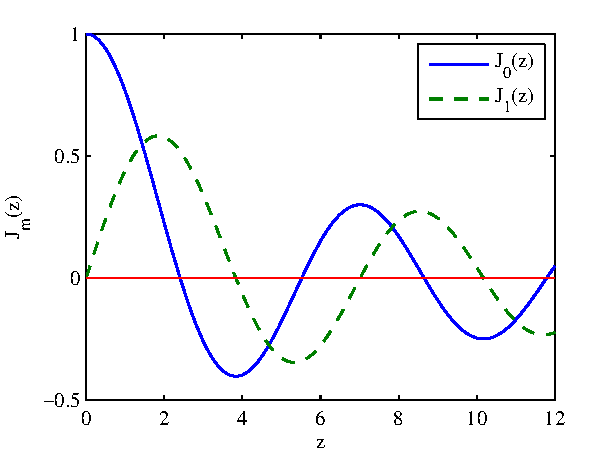
\includegraphics[width=\textwidth]{chp-2_bessel_j}
    (a) 子图a图题子图a图题子图a图题
  \end{minipage}%
  \begin{minipage}[t]{0.5\textwidth}
    \centering
    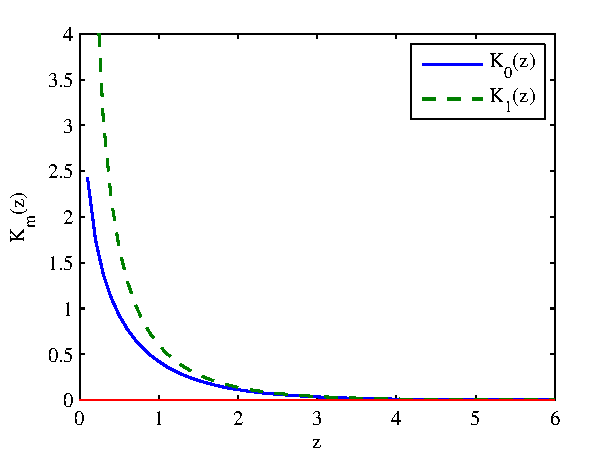
\includegraphics[width=\textwidth]{chp-2_bessel_k}
    (b) 子图b图题子图b图题子图b图题
  \end{minipage}
    \Figcaption{两个并排图形}\label{fig-dbfig}
 \end{figure}
\end{comment}

\section{问题构建}\label{section2-2}
\subsection{系统及信道模型}\label{section2-2-1}
我们考虑了一种上行链路空地一体化通信场景,在这种场景中,众多车对无人机(V2U)小区覆盖在一个宏蜂窝之下。
如图 \ref{天地网络系统模型} 所示,无人机固定悬停并部署在交通拥堵路段,负责接收其覆盖范围内车辆的信号并
将其发送到基站(BS)。值得注意的是,所有无人机都是双工的,配备有接收天线和发射天线,因此接收和发射过程
可以同时完成。通信中的CUE和VUE集合分别索引为$\mathcal{S}_0:= \{0\}$ 和$\mathcal{S}_l:=\{1, 2,..., N\}$ 。
为了提高频谱利用率,实现多用户联合通信,V2U 通信重复使用了CUE 的上行信道。但是会产生严重的多用户干扰,
限制了信号链路的通信。如图 \ref{天地网络系统模型} 所示,信号链路(蜂窝链路和同信道 V2U 链路)和干扰链路(CUE-V 链路、V-BS 链
路和 V2U 干扰链路)被区分开来。

假设无人飞行器的飞行高度为 $H_n$,则 VUE$_{k}$ 与 UAV$_{n}$ 之间的距离为:
\begin{eqnarray}\label{E2-1}
h_{k,n}=\sqrt{H_n^2+(\|W_k-W_n\|)^2},           &k\in \mathcal{N}, n\in \mathcal{N}
\end{eqnarray}
其中 $W_k$ 和 $W_n$ 是 VUE$_{k}$ 与 UAV$_{n}$的位置信息,  CUE 与BS之间的距离为:
\begin{eqnarray}\label{E2-2}
h_{0,0}=\sqrt{H_0^2+(\|W_0-W_{BS}\|)^2},
\end{eqnarray}
其中,$W_0$ 和 $W_{BS}$ 为 CUE 和 BS 的位置,$H_0$ 为 BS 上信号接收器的垂直高度。VUE$_{k}$ 与 BS 之间的距离为 $h_{k,0}$,CUE 与 UAV$_{n}$ 之间的距离为 $h_{0,n}$。$h_{k,0}$和$h_{0,n}$的表达式类似于 \eqref{E2-1}和 \eqref{E2-2}。

\begin{figure}[H]
\centering
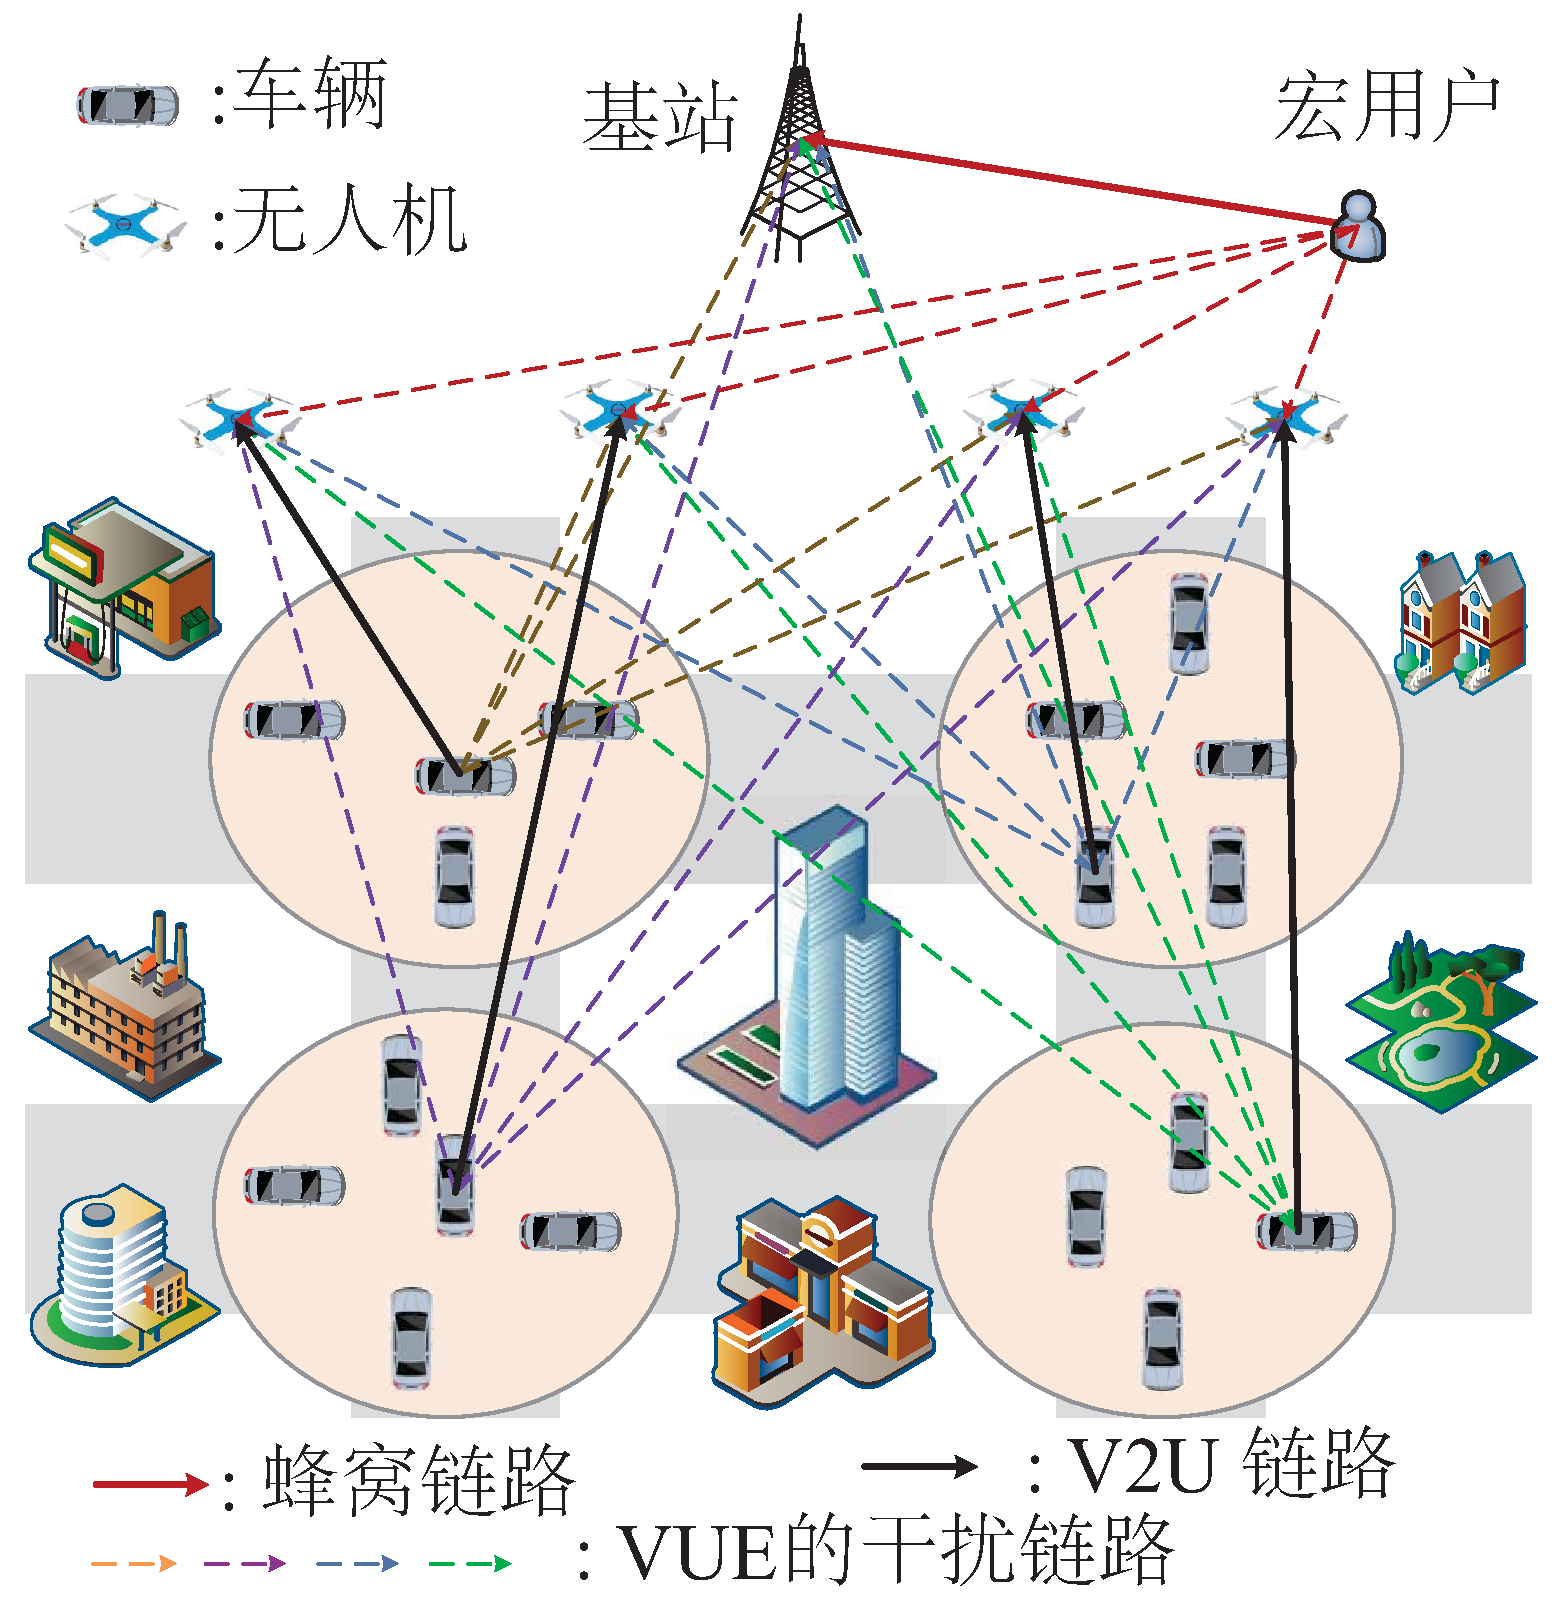
\includegraphics[width=10cm]{figures//chap2//china1.pdf}
\caption{天地网络系统模型}
\label{天地网络系统模型}
\end{figure}
\begin{comment}
\begin{figure}[hptb!]
 \centering\small
 \includegraphics[width=0.6\textwidth]{figures//chap2//cchina1.pdf}
 \Figcaption{无人机的系统模型}\label{sysjktemuav}
\end{figure}
\end{comment}

蜂窝链路和同信道 V2U 链路的大规模衰落可分别表示为:
\begin{eqnarray}\label{E2-3}
g_{0,0}=L_{0,0}h_{0,0}^{-\alpha},
\end{eqnarray}
\begin{eqnarray}\label{E2-4}
g_{n,n}=L_{k,n}h_{k,n}^{-\alpha},          &k, n\in \mathcal{N}, k=n
\end{eqnarray}
其中,$L_{0,0}$ 和 $L_{n,n}$ 是蜂窝链路和同信道 V2U 链路的阴影衰减效应。$\alpha$ 是路径损耗指数。虽然车辆与无人机之间的传输链路可视为借助无人机在道路上空进行的 LoS 通信,
但仍存在一些影响信道增益的因素,如通信终端的相对移动、信道估计误差以及不可避免的信道不确定性。因此,小尺度衰落不容忽视。根据 \cite{CCO},它遵循截断指数分布。为了描述信
道增益的不确定性,引入了一个参数 $G$,$G$ 是一个独立的同分布随机变量,其概率密度函数为 $f_G (x)=e^{-x}$ 。信号链路 $n$ 的实时信噪比(SINR)可表示为:
\begin{eqnarray}\label{E2-5}
\gamma_{n}(p_n)=\frac{p_{n}G g_{n,n}}{I_n}, k\in\mathcal{N},n\in\mathcal{N},
\end{eqnarray}
其中,$g_{n,n}$ 是给定时隙内的估计增益。同信道 V2U 链路 $n$ 的干扰可视为测量值,其表达式为:
\begin{eqnarray}\label{E2-6}
I_n=p_0 g_{0,n}+\!\!\!\sum\limits_{k=1,k\neq n}^N\!\!\!\! p_k g_{k,n}+\delta^2, \quad k\in\mathcal{N},n\in\mathcal{N},
\end{eqnarray}
其中,$p_k$ 表示第 $k$ 个 VUE 的传输功率。$p_0$ 是 CUE 的传输功率。$\delta^2$ 是噪声干扰。

为处理不确定参数 $G$,确保 V2U 通信质量,我们引入了以下中断概率约束、
\begin{eqnarray}\label{E2-7}
\textrm{Pr}\left\{\gamma_{n} \leq \gamma_{th}\right\}\geq1-\varepsilon,\quad  n\in\mathcal{N}
\end{eqnarray}
其中,$\gamma_{n}$ 表示第 $n$ 个同频 V2U 链路的瞬时 SINR。$\gamma_{th}$是事先给定的阈值,代表目标 SINR。$\varepsilon$ 是中断概率阈值,$\varepsilon \in (0,1)$ 。

考虑了不确定的信道增益,并使用遍历容量来显示网络性能。
\begin{eqnarray}\label{E2-8}
R_{er}=\int_{0}^{\infty} W \log(1+\gamma_{n})\Pr(\gamma_{n})\, d(\gamma_{n}),
\end{eqnarray}
其中,$W$ 是复用信道的带宽,$\Pr(\gamma_{n})$ 是 $\gamma_{n}$ 的概率分布函数。
根据詹森不等式认为
\begin{eqnarray}\label{E2-9}
 \begin{array}{lll}
&\!\!\!\!\!\!\mathbb{E}\{W \log(1+\gamma_{n}\}=\int_{0}^{\infty} W \log(1+\gamma_{n})\ \Pr(\gamma_{n})\, d(\gamma_{n})\\
&\quad\quad\quad\quad\quad\quad\quad\!\!<W\log(1+\mathbb{E}\{\gamma_{n}\})\\
&\quad\quad\quad\quad\quad\quad\quad\!\!=W\log(1+\bar{\gamma}_{n}),
 \end{array}
\end{eqnarray}
其中 $\bar{\gamma}_{n}\!=\mathbb{E}\{\!\frac{p_{n}G g_{n,n}}{I_n}\}
\!=\!\frac{p_{n}g_{n,n}}{I_n}$. 这也是香农容量是遍历容量的上限,通过信道编码技术可以使遍历容量接近上限。
因此,根据香农定理计算出的 VUE 的确定性等效传输速率为:
\begin{eqnarray}\label{E2-10}
R_{n}=W\log(1+\bar{\gamma}_{n}(p_n)),\quad  n\in\mathcal{N}.
\end{eqnarray}
\subsection{博弈论问题}\label{section2-2-1}
在空地一体化异质车载网络(AGHVN)中,频谱所有者 CUE 可以对干扰进行定价,并将 VUE 的收费作为其利润。在 V2U 小区中,VUE 的效用是传输速率与购买干扰成本之间的差额。
考虑到 CUE 和 VUE 都是自私自利的,它们都愿意为自己的利益而竞争。因此,数学框架自然符合 Stackelberg 博弈模型,其中 CUE 和 VUE 分别是领导者和追随者。此外,还考虑了
 CUE 的通信约束。第$n_{th}$ 个V2U 单元的下子博弈可表述为:
\begin{comment}
\begin{eqnarray}\label{11}
\end{comment}

\begin{align}
&P_1: \max\limits_{p_{n}} U_{n}=R_{n}\!\!-c_{n} p_n g_{n,0}                                                          \label{E2-11}\\
&\text { s.t. }
\quad \!\!\!\!\! \textrm{Pr}\left\{\gamma_{n}(p_n) \geq \gamma_{th}\right\}\geq1-\varepsilon  \tag{\ref{E2-11}{-1}}  \label{E2-11-1}\\
& \quad \quad \quad \!\!\!\!\! 0\leq p_n\leq p_{n,\textrm{max}}                               \tag{\ref{E2-11}{-2}}  \label{E2-11-2}
\end{align}
其中,$U_{n}$ 是第 $n$ 个 V2U 信号链路的效用,$p_{n,\textrm{max}}$ 是功率的上限。

作为领导者,价格策略应保证每个用户都有正收益。因此,蜂窝网络的上子博弈可以表述为
\begin{align}
&P_2: \max\limits_{\mathbf{c}} U_0=\sum\limits_{n=1}^N c_{n} p_n(c_{n}) g_{n,0}                    \label{E2-12}\\
& \text { s.t. }
\quad \!\!\!\!\! R_{n}\{p_n(c_{n})\} \geq c_{n} p_n(c_{n}) g_{n,0}          \tag{\ref{E2-12}{-1}}  \label{E2-12-1}\\  %信噪比中断概率约束
& \quad \quad \quad \!\!\!\!\! 0\leq c_n\leq c_{n,\textrm{max}}             \tag{\ref{E2-12}{-2}}  \label{E2-12-2}  %功率阈值
\end{align}
其中,$U_{0}$ 是蜂窝链接的效用。$c_{n,\textrm{max}}$ 是价格上限。

此外,通过寻找子博弈的纳什均衡(NE),可以得到所提出的斯塔克尔伯格博弈的博弈均衡(GE)。关于(NE)和(GE)的详细描述请参阅 \cite{RAI}。
\section{博弈问题求解}\label{section2-3}
\subsection{概率约束的转化}\label{section2-3-1}
从 \eqref{E2-6}和 \eqref{E2-7}可以看出,中断概率约束可以表示为:
\begin{equation}\label{E2-13}
\textrm{Pr}\left\{\frac{p_{n}G g_{n,n}}{I_n} \geq \gamma_{th}\right\}\geq1-\varepsilon.
\end{equation}
由于 $G$ 的概率密度函数为 $f_G (x)=e^{-x}$,因此可通过变量积分得到:
\begin{equation}\label{E2-14}
\int_{0}^{\frac{\gamma_{th}I_{n}}{p_n g_{n,n}}} e^{-x}\, dx\leq\varepsilon.
\end{equation}

可以认为:
\begin{equation}\label{E2-15}
\frac{p_n g_{ n,n}}{I_{n}}\geq\frac{-\gamma_{th}}{\ln(1-\varepsilon)}.
\end{equation}

因此,中断概率约束的确定性表达式可求得如下,
\begin{equation}\label{E2-16}
\frac{-\gamma_{th} I_{n}}{\ln(1-\varepsilon)}-p_n g_{n,n}\leq0,\quad\forall n\in\mathcal{N}.
\end{equation}
\subsection{求解下层子问题}\label{section2-3-2}
通过转换概率约束条件,可以得到一个资源分配的确定性优化问题。
\begin{align}
&P_3: \max \limits_{p_{n}} R_{n}\!\!-c_{n} p_n g_{n,0}               \label{E2-17}\\
&\text { s.t. }
 \quad \!\!\!\!\! \frac{-\gamma_{th} I_{n}}{\ln(1-\varepsilon)}-p_n g_{n,n}\leq0 \tag{\ref{E2-17}{-1}} \label{E2-17-1}\\ %信噪比中断概率约束
& \quad \quad \quad \!\!\!\!\! 0\leq p_n\leq p_{n,\textrm{max}}                  \tag{\ref{E2-17}{-2}} \label{E2-17-2}  %功率阈值
\end{align}

由于 $P_3$ 是一个标准的凸优化问题,因此要构造拉格朗日函数来求解最优幂。 \eqref{E2-17} 的拉格朗日函数表述为
\begin{eqnarray}\label{E2-18}
\begin{array}{lll}
\textit{L}_n(p_n, \lambda_n)=R_{n}\!\!-\!\!c_{n} p_n g_{n,0}\!\!-\!\!\lambda_n \left(\frac{-\gamma_{th} I_{n}}{\ln(1-\varepsilon)}-p_n g_{n,n}\right),
\end{array}
\end{eqnarray}
其中,$\lambda_n$ 是拉格朗日乘数,$\lambda_n \geq 0$。

使用子梯度法,可以得到拉格朗日乘数的迭代更新表达式,
\begin{equation}\label{E2-19}
\begin{array}{lll}
     \lambda_n^{(t+1)}=[\lambda_n^{(t)}\!\!+\!K_{\lambda}^{(t)}(\frac{-\gamma_{th} I_{n}^{(t)}}{\ln(1-\varepsilon)}-p_n^{(t)} g_{n,n})]^+,
\end{array}
\end{equation}

其中 $I_{n}^{(t)}=$$p_0 g_{0,n}+\sum_{k=1,k\neq n}^N p_k^{(t)} g_{k,n}$。
$P3$ 的卡鲁什-库恩-塔克(KKT)条件为,
\begin{equation}\label{E2-20}
\begin{array}{rl}
\left\{
\begin{array}{lll}
     \frac{\partial \textit{L}_n(p_n, \lambda_n)}{\partial p_n}\!=\!\frac{W g_{n,n}}{p_n g_{n,n}+I_n}\!-\!c_n g_{n,0}\!-\!\lambda_n g_{n,n}\!=\!0\\
     \lambda_n \big(\frac{-\gamma_{th} I_{n}}{\ln(1-\varepsilon)}-p_n g_{n,n}\big)=0\\
     \lambda_n \geq 0
\end{array}
\right.
\end{array}
\end{equation}

每个 VUE 的最优传输功率为,
\begin{equation}\label{E2-21}
\begin{array}{*{21}{ll}}
 p_n^{*}=\frac{W}{c_n g_{n,0}-\lambda_n^{*}g_{n,n}}-\frac{I_n^{*}}{g_{n,n}}.
\end{array}
\end{equation}

此外,迭代表达式如下,
\begin{eqnarray}\label{E2-22}
 \begin{array}{lll}
p_n^{(t+1)}=\frac{W}{c_n g_{n,0}-\lambda_n^{(t+1)}g_{n,n}}-\frac{I_n^{(t+1)}}{g_{n,n}}.
\end{array}
\end{eqnarray}

要证明 \eqref{E2-21}是 GE,就要讨论 NE 的存在性和唯一性。

存在性: 正如 \cite{GT} 中所指出的,在堆积尔伯格子博弈 \eqref{E2-10}中存在一个NE,条件是

1) $\mathbf{P}$ 是某个欧几里得空间 $\mathcal{R}^N$ 的非空凸紧凑子集,

2) $U_{\textrm{n}}(p_n)$ 在 $\mathbf{P}$ 中是连续的,在 $p_n$ 中是凹的。

\begin{proof}
1) 功率策略空间为 $\mathbf{P}=\{p_n:0\leq p_n \leq p_{n,\textrm{max}}\}$, 它是欧几里得空间 $\mathcal{R}^N$ 的一个非空、凸和紧凑子集。
2) 得到效用关于 $p_n$ 的一阶导数、
\begin{equation}\label{23}
\frac{\partial U_{n}}{\partial p_n}=\frac{Wg_{n,n}}{p_n g_{n,n}+I_n}-c_ng_{n,0}.
\end{equation}
得到关于 $p_n$ 的二阶导数、
\begin{equation}\label{24}
\frac{\partial^2 U_{n}}{\partial p_n^2}=-\frac{W(g_{n,n})^2}{\big(p_n g_{n,n} +I_n\big)^2}<0.
\end{equation}
由于 $U_{\textrm{n}}(p_n)$ 相对于 $p_n$ 的二阶导数总是小于 0,所以 $U_{\textrm{n}}(p_n)$ 在 $p_n$ 中是凹的。因此,在斯塔克尔伯格子博弈 \ref{E2-10}中存在一个NE 。
\end{proof}\par

唯一性: 当$g_{n,n}$$>$$\sum\limits_{k=0,k\neq n}^N g_{k,n}$时,在拟议的斯塔克尔伯格子博弈中,NE是唯一的。

\begin{proof}
让 $p_{-n}(t)=[p_k(t)]_{k\in\mathcal{K},k\neq n}$,那么
%\begin{eqnarray}\label{25}
%\begin{array}{lll}。
%G_{-n}p_{-n}(t)=\sum\limits_{k=1,k\neq n}^N g_{k,n}p_k(t)、
%\end{array}
%\end{eqnarray}
\begin{equation} \label{E2-25}
G_{-n}p_{-n}(t)=\sum\limits_{k=1,k\neq n}^N g_{k,n}p_k(t)
\end{equation}
其中 $G_{-n}=[g_{k,n}]_{k\in\mathcal{N},k\neq n}^T$ \par
定义 $\Delta p_{n}(t)=p_{n}(t)-p_{n}^*$ ,我们得到
\begin{eqnarray}\label{E2-26}
\hspace{-0.2cm}
 \begin{array}{lll}
&\!\!\!\!\!\!\!|\Delta p_{n}(t+1)|=|p_{n}(t+1)-p_{n}^*|\\
&\quad \quad \quad \quad =\Big|\frac{\sum_{k=0,k\neq n}^N g_{k,n}(p_k^{(t)}-p_k^*)}{g_{n,n}}\Big|\\
&\quad \quad \quad \quad =\Big\|\frac{\sum_{k=0,k\neq n}^Ng_{k,n}}{g_{n,n}}\Big\|_\infty \big\|\sum_{k=0,k\neq n}^N\Delta p_{k}(t)\big\|_\infty.
\end{array}
\end{eqnarray}

一般情况下,V2U 信号链路的信道增益大于干扰链路,所以 $g_{n,n}$$>$$\sum_{k=0,k\neq n}^N g_{k,n}$ 是可行的。然后,我们可以得到 $\|\frac{G_{-n}}{g_{n,n}}\|$$<$$1$ 。
根据$l_\infty-$norm的定义,我们知道$\big\|\sum_{k=0,k\neq n}^N\Delta p_{k}(t)\big\|_\infty$$=$$\max [\Delta p_{k}(t)]_{k\in\mathcal{N},k\neq n}$。因此,
$\delta p_{n}(t+1)$ 在迭代一段时间后可以趋近于零,而 $p_{n}(t+1)$ 可以趋近于唯一的最优点 $p_{n}^*$。因此,在 Stackelberg 子博弈中,NE 是唯一的。
\end{proof}
\subsection{求解上层子问题}\label{section2-3-3}
由\ref{section2-3-2}得到的VUE 的最优传输功率 $p_n$可用来求解上层子问题。
在上层网络中,根据 VUE 的最优传输功率 $p_n$,原来的上层子博弈可以重写为,
\begin{align}
& \!\!\!\!\!\!\!P_4:\max\limits_{\mathbf{c}} \quad \sum\limits_{n=1}^N c_{n} p_n(c_{n}) g_{n,0}                   \label{E2-27}  \\
\text { s.t. }
& W\log(1+\frac{p_{n}(c_{n}) g_{n,n}}{I_n}) \geq c_{n} p_n(c_{n}) g_{n,0}         \tag{\ref{E2-27}{-1}} \label{E2-27-1}\\  %信噪比中断概率约束
& p_n(c_{n})\!\!=\!\!\frac{W}{c_n g_{n,0}-\lambda_n g_{n,n}}-\frac{I_n}{g_{n,n}}  \tag{\ref{E2-27}{-2}} \label{E2-27-2}\\ %功率阈值
& 0\leq c_n\leq c_{n,\textrm{max}}                                                \tag{\ref{E2-27}{-3}} \label{E2-27-3}
\end{align}

每个子问题的拉格朗日函数表示如下,
\begin{comment}
\begin{eqnarray}\label{28}
 \begin{array}{lll}
&\!\!\!\textit{L}_n(c_n, \mu_n)=(1-\mu_n)c_{n} g_{n,0}\left(\frac{W}{c_n g_{n,0}-\lambda_n g_{n,n}}-\frac{I_n}{g_{n,n}}\right)\\
&\quad \quad \quad \quad \quad +\mu_n W \log\left(\frac{W g_{n,n}}{I_n (c_n g_{n,0}-\lambda_n g_{n,n}) }\right) ,
\end{array}
\end{eqnarray}
\end{comment}
\begin{eqnarray}\label{E2-28}
\begin{array}{lll}
\!\!\!\!\textit{L}_n(c_n, \mu_n)=(1-\mu_n)c_{n} g_{n,0}\left(\frac{W}{c_n g_{n,0}-\lambda_n g_{n,n}}-\frac{I_n}{g_{n,n}}\right)
+\mu_n W \log\left(\frac{W g_{n,n}}{I_n (c_n g_{n,0}-\lambda_n g_{n,n}) }\right) ,
\end{array}
\end{eqnarray}
其中,
\begin{comment}
\begin{eqnarray}\label{29}
 \begin{array}{lll}
&\!\!\!\mu_n^{(t+1)}=\Big[\mu_n^{(t)}\!\!+\!K_{\mu}^{(t)}\big(c_{n}^{(t)} g_{n,0}(\frac{W}{c_n^{(t)} g_{n,0}-\lambda_n g_{n,n}}-\frac{I_n}{g_{n,n}})\\
&\quad \quad \quad \quad \quad -\mu_n^{(t)} W \log(\frac{W g_{n,n}}{I_n (c_n^{(t)} g_{n,0}-\lambda_n g_{n,n}) })\big)\Big]^+ .
\end{array}
\end{eqnarray}
\end{comment}
\begin{eqnarray}\label{E2-29}
\begin{array}{lll}
\!\!\!\mu_n^{(t+1)}=\Big[\mu_n^{(t)}\!\!+\!K_{\mu}^{(t)}\big(c_{n}^{(t)} g_{n,0}(\frac{W}{c_n^{(t)} g_{n,0}-\lambda_n g_{n,n}}-\frac{I_n}{g_{n,n}})-\mu_n^{(t)} W \log(\frac{W g_{n,n}}{I_n (c_n^{(t)} g_{n,0}-\lambda_n g_{n,n}) })\big)\Big]^+ .
\end{array}
\end{eqnarray}

通过使用卡鲁什-库恩-塔克(KKT)条件的类似求解过程,干扰价格的迭代表达式为,
\begin{eqnarray}\label{E2-30}
 \begin{array}{lll}
\!\!\!\!c_n^{(t+1)}\!\!\!=\!\!\frac{g_{n,n}}{g_{n,0}}\!\!\left(\!\!\frac{ \sqrt{(W\mu_n^{(t)})^{2}\!-4W\lambda_n(\mu_n^{(t)}\!\!-\!1)^2I_n}}{(\mu_n^{(t)}-1)I_n}\!\!+\!\! (\lambda_n\!\!\!-\!\!\frac{W\mu_n^{(t)}}{2(\mu_n^{(t)}\!\!-\!1)I_n})\!\!\right).\!\!\!\!
\end{array}
\end{eqnarray}
根据 \eqref{E2-30} 可以计算干扰价格的最优值 $c_{n}^{(t+1)}$。

$c_n$的GE证明与上一小节 \ref{section2-3-2} 中$p_n$的证明类似。此处省略相应内容。
\section{算法与仿真验证}\label{section2-4}
\subsection{斯塔克尔伯格博弈的迭代算法}\label{section2-4-1}
本节提出了一种基于斯台克尔伯格博弈的鲁棒资源分配算法来解决优化问题 \eqref{E2-11}和 \eqref{E2-12}。该算法如下所示,

\begin{tabular*}{\hsize}{@{\extracolsep{\fill}}l l l l}
    \toprule
    算法2-1基于斯坦克尔伯格博弈的鲁棒资源分配算法                                                             \\
    \midrule
    Step1: 开始。                                                                                            \\
    Step2: 初始化功率$p_{n}(0)$ 和干扰价格$c_{n}(0)$                                                         \\
    Step3: 设置 $t=1$,$T=20$,$p_{n}(0)$ 为可行区域内的任意一点,且$0\leq p_{n}(0)\leq p_{n,\textrm{max}}$。\\ %, $n \in [1,2,...,N]$
    Step4: 设置$\lambda_{n}>0$ , $\mu_{n}>0$, $K_{\lambda} >0$,$K_{\mu} >0。$                             \\
    Step5: 根据  \eqref{E2-19} 更新乘子 $\lambda_{n}$。                                                         \\
    Step6: 更新第 $n$ 个 VUE 收到来自 BS 的干扰价格,然后根据 \eqref{E2-22}计算 $p_{n}^{(t+1)}$                 \\
    Step7: BS 收到 D2D-V 用户的最优响应函数和反馈信息后,根据 \eqref{E2-29})更新乘子 $\mu_{n}^{(t+1)}$         \\
    Step8: 根据 \eqref{E2-30} 计算干扰价格 $c_{n}^{(t+1)}$。                                                    \\
    Step9: 重复执行Step5至Step8,直到满足$p_{n}$ 和$c_{n}$ 收敛并且 $t<T$                                    \\
    Step10:设置 $t=t+1$                                                                                      \\
    Step11:结束。                                                                                            \\
    \bottomrule
\end{tabular*}
\subsection{仿真分析}\label{section2-4-2}
本节将进行数值模拟,以评估基于鲁棒的斯塔克尔伯格博弈的资源分配算法的性能。在半径为 $500m$ 的 BS 覆盖范围内,模拟了一个包含 1 个 CU 和 9 个 V2U 集群的简化车辆通信模型,
用于模拟异构通信场景。表 \ref{biao2-1} 列出了相应的系统参数。

\begin{table}[htbp!]
 \centering\small
 \renewcommand\arraystretch{1.5}   %latex三线表中各行间隔
 \Tablecaption{系统仿真参数}\label{biao2-1}
\begin{tabular*}{\hsize}{@{\extracolsep{\fill}}c c c c}
 \toprule
    \qquad\qquad \zihao{5}符号          &\qquad\qquad 参数                        & \qquad\qquad 数值         \\
 \midrule
    \qquad\qquad $R$           &\qquad\qquad \zihao{5}基站的通信范围              & \qquad\qquad 500 m        \\
    \qquad\qquad $H_n$         &\qquad\qquad {\CJKfamily{song}\zihao{5} 无人机的巡航高度}            & \qquad\qquad 30 m         \\
    \qquad\qquad $H_0$         &\qquad\qquad {\zihao{5} 基站上信号接收器的垂直高度}  & \qquad\qquad 30 m         \\
    \qquad\qquad $W$           &\qquad\qquad 信道带宽                    & \qquad\qquad 10 MHz       \\
    \qquad\qquad $L$           &\qquad\qquad 阴影衰落效果                & \qquad\qquad 0.9          \\
    \qquad\qquad $\alpha$      &\qquad\qquad 路径损耗指数                & \qquad\qquad 1.4          \\
    \qquad\qquad $\delta^2$    &\qquad\qquad 噪声方差                    & \qquad\qquad -30 dBm      \\
    \qquad\qquad $p_{i,max}$   &\qquad\qquad 最大功率                    & \qquad\qquad 0.01 W       \\
    \qquad\qquad $I_{th}$      &\qquad\qquad 干扰阈值                    & \qquad\qquad ${10}^{-3}$  \\
    \qquad\qquad $\varepsilon$ &\qquad\qquad 中断概率阈值                & \qquad\qquad 0.1          \\
 \bottomrule
 \end{tabular*}
\end{table}
基于鲁棒的斯塔克尔伯格博弈的资源分配算法的收敛性能如图 \ref{F2} 和图 \ref{F3}所示。九个 VUE 的发射功率用 $p_{1}-p_{9}$ 表示,
价格用 $c_{1}-c_{9}$ 表示。如图 \ref{F2} 所示,功率在第七步收敛到最优值。根据图 \ref{F3},VUE 的非均匀价格逐渐趋于稳定,最终达到收敛。
因此,图 \ref{F2} 和图 \ref{F3} 中的结果表明,所提出的基于鲁棒博弈的资源分配算法是快速有效的。

\begin{figure}[H]
\centering
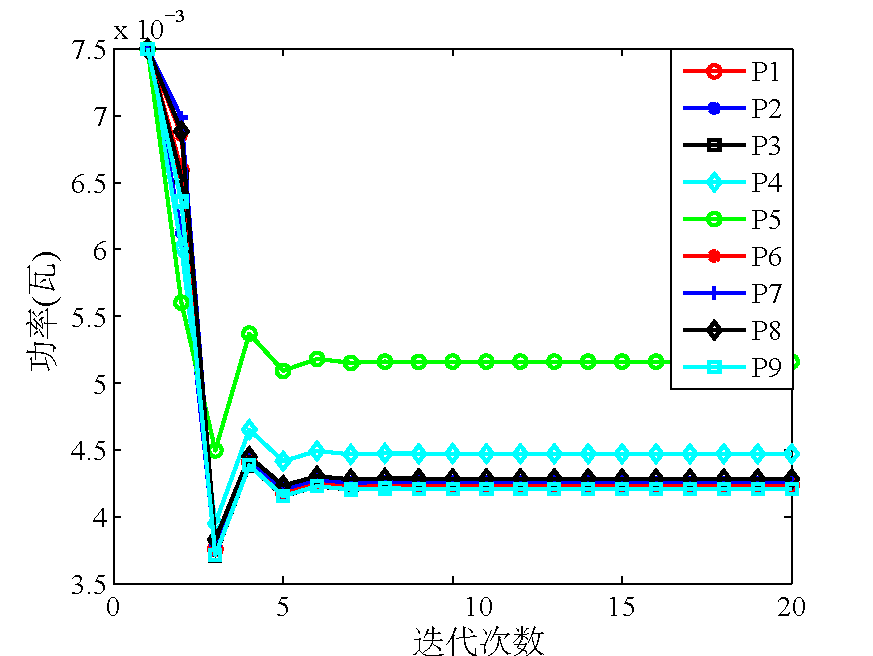
\includegraphics[width=10cm]{figures//chap2//2.pdf}
\caption{功率收敛性能}
\label{F2}
\end{figure}
\begin{figure}[H]
\centering
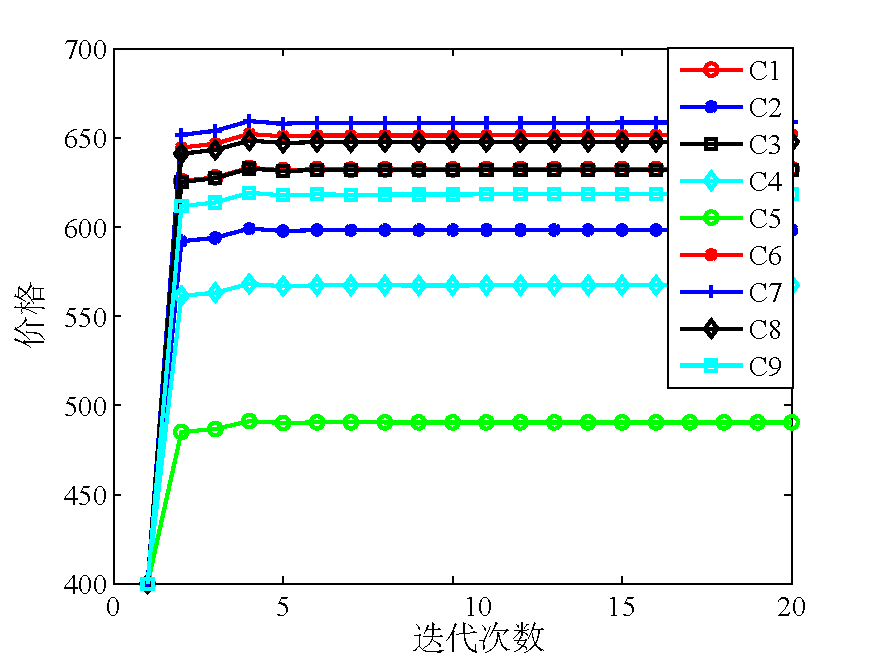
\includegraphics[width=10cm]{figures//chap2//3.pdf}
\caption{价格收敛性能}
\label{F3}
\end{figure}

为了进一步验证所提算法的性能,图 \ref{F4} 和图 \ref{F5} 完成了对系统鲁棒性和传输速率的验证。在异质通信场景中,严重的多用户干扰会影响用户的信号传输,甚至造成中断。
如图 \ref{F4} 所示,当 $\varepsilon$ 在 0.1 到 0.4 之间变化时,用户的实际中断概率总是小于给定的阈值。结果证实,不仅实现了有效的干扰管理,还保证了传输的鲁棒性。
通过与 \cite{PCID}和基线(目标和实际中断概率相等)比较,本文所有用户的实际中断概率都是最低的。这进一步说明本文提出的基于鲁棒博弈的算法在信道不确定性较高的实际场景中更加稳定。
\begin{figure}[H]
\centering
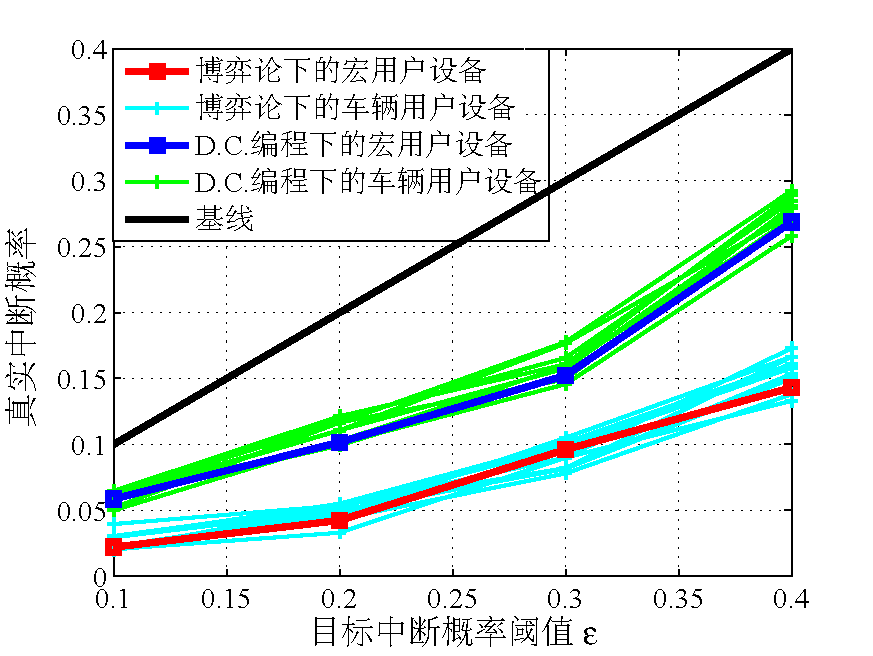
\includegraphics[width=10cm]{figures//chap2//4.pdf}
\caption{中断概率对此}
\label{F4}
\end{figure}


\begin{figure}[H]
\centering
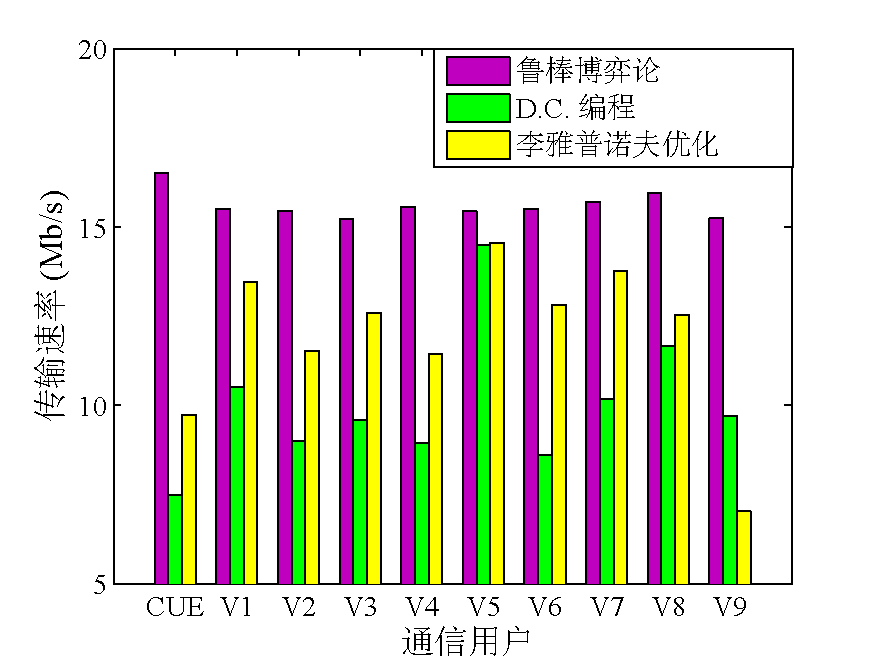
\includegraphics[width=10cm]{figures//chap2//5.pdf}
\caption{传输速率对比}
\label{F5}
\end{figure}

如图 \ref{F5} 所示,本文中 CUE 和 VUE 的传输速率比 \cite{PCID}和 \cite{ACAR}更均衡。这是因为我们构建了一个非合作博弈框架,在这个框架中,VUE 都是自私的,
都在为自己的利益而竞争。在原问题 \eqref{E2-12}和 \eqref{E2-13}中,价格是实现 VUE 之间平衡的关键变量。当一个 VUE 通过增加功率来提高传输速率时,它将受到来自 BS 的更
多干扰费的惩罚。通过多轮博弈,每个用户都达到了自己最满意的状态,因此用户的传输速率得到了很好的平衡,也高于 \cite{PCID}和 \cite{ACAR}中的传输速率。
\section{本章小结}\label{section2-5}
在章节中,我们提出了一种基于博弈的鲁棒的资源分配算法,以实现 AGHVN 中的有效信息传输。该算法以用户间的博弈关系为核心,制定了实时功率分配和定价策略,
在新颖的优化方案中实现了用户利益的最大化。具体而言,为了保证系统的鲁棒性,引入了概率约束,以确保用户服务的可靠性和稳定性。由于信道不确定性的存在,
概率形式非凸且难以处理,因此在凸优化过程中采用了指数积分法。根据仿真结果,幂值和价格在几步内收敛到最优值。我们还可以得出结论,斯塔克尔伯格博弈优化方
案表现出更好的鲁棒性。因此,所提出的基于鲁棒博弈的资源分配算法在具有复杂多用户干扰和信道不确定性的空地一体化异构车载通信场景下是有效的。






















\begin{comment}
\begin{verbatim}
\begin{figure}[hptb!]
  \centering\small
  \begin{minipage}[t]{0.5\linewidth}
    \centering
    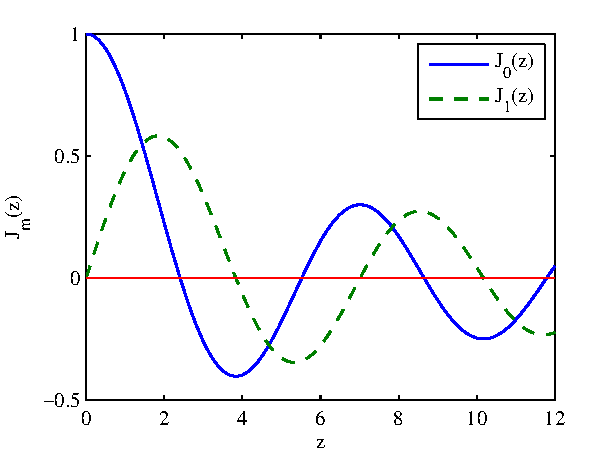
\includegraphics[width=\textwidth]{chp-2_bessel_j}
    (a) 子图a图题
  \end{minipage}%
  \begin{minipage}[t]{0.5\textwidth}
    \centering
    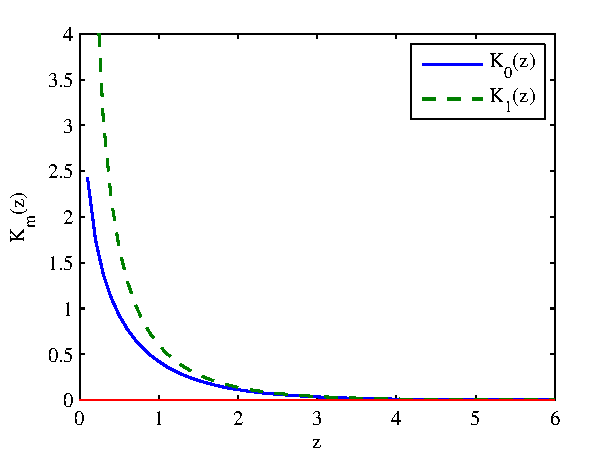
\includegraphics[width=\textwidth]{chp-2_bessel_k}
    (b) 子图b图题
  \end{minipage}  \\
  \begin{minipage}[t]{0.5\textwidth}
    \centering
    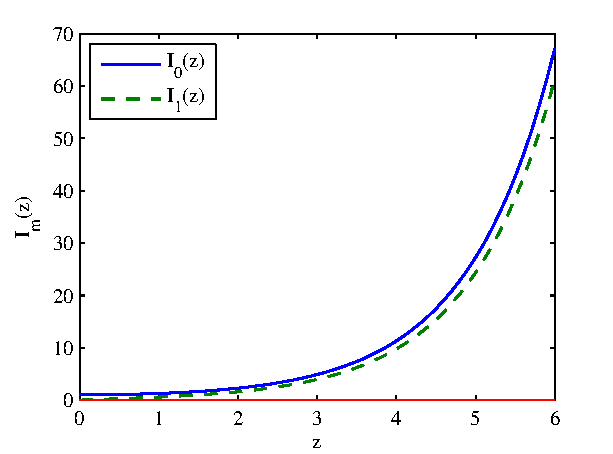
\includegraphics[width=\textwidth]{chp-2_bessel_i}
    (c) 子图c图题子图c图题子图c图题
  \end{minipage}%
  \begin{minipage}[t]{0.5\textwidth}
    \centering
    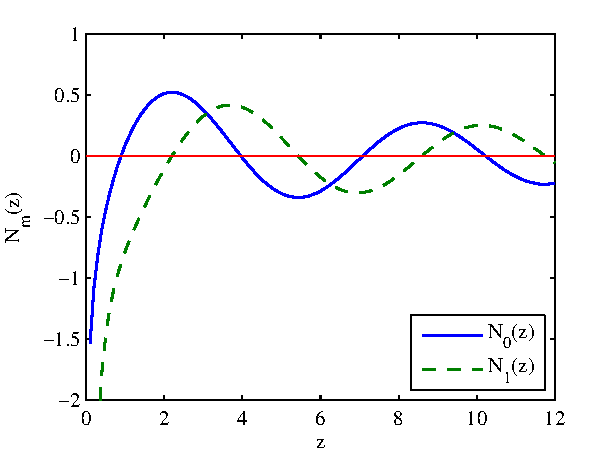
\includegraphics[width=\textwidth]{chp-2_bessel_n}
    (d) 子图d图题子图d图题子图d图题
  \end{minipage}
\Figcaption{贝塞尔函数}  \label{fig-bessel-function}
\end{figure}
\end{verbatim}
注意其中与一对并排图形不同的地方,加入了换行命令“$\backslash\backslash$”。
最终效果如图\ref{fig-bessel-function}所示。
\begin{figure}[hptb!]
  \centering\small
  \begin{minipage}[t]{0.5\linewidth}
    \centering
    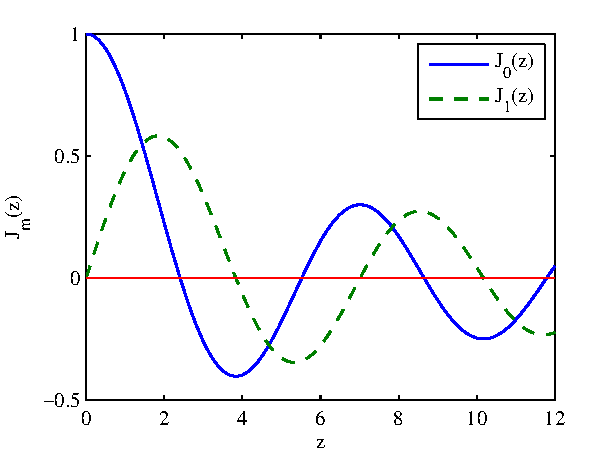
\includegraphics[width=\textwidth]{chp-2_bessel_j}
    (a) 子图a图题
  \end{minipage}%
  \begin{minipage}[t]{0.5\textwidth}
    \centering
    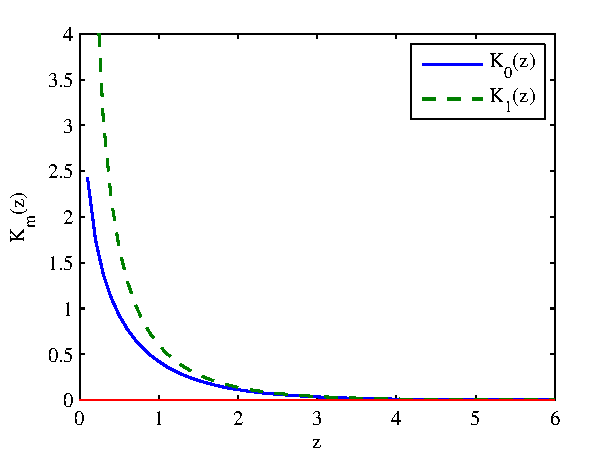
\includegraphics[width=\textwidth]{chp-2_bessel_k}
    (b) 子图b图题
  \end{minipage}  \\
  \begin{minipage}[t]{0.5\textwidth}
    \centering
    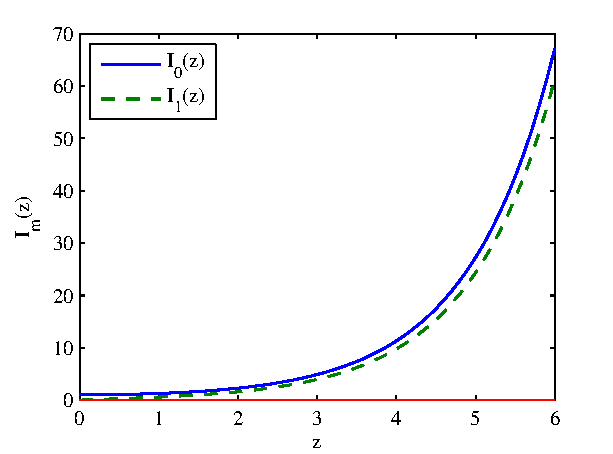
\includegraphics[width=\textwidth]{chp-2_bessel_i}
    (c) 子图c图题子图c图题子图c图题
  \end{minipage}%
  \begin{minipage}[t]{0.5\textwidth}
    \centering
    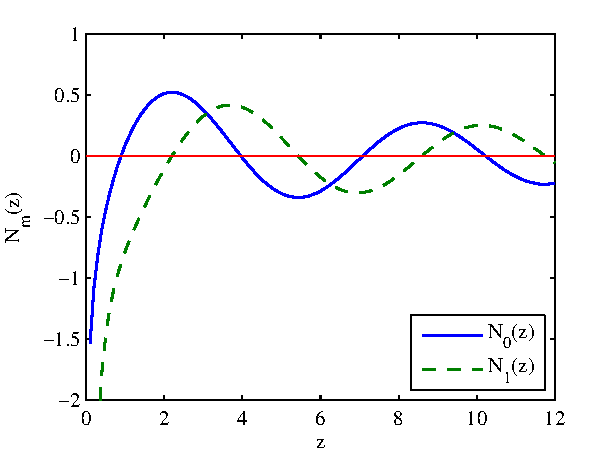
\includegraphics[width=\textwidth]{chp-2_bessel_n}
    (d) 子图d图题子图d图题子图d图题
  \end{minipage}
\Figcaption{贝塞尔函数}  \label{fig-bessel-function}
\end{figure}

其它类似的多个图形并排或者堆叠均可以灵活的运用minipage照猫画虎获得。

\section{图题}\label{section2-4}
其实上边的例子中已经包含了图题的引用命令\verb|\Figcaption|。
例如图\ref{fig-bessel-function}中:
\begin{verbatim}
    \Figcaption{贝塞尔函数}\label{fig-bessel-function}
\end{verbatim}
为当前的图形添加中文图题“贝塞尔函数”。同时添加标签“fig-bessel-function”。对图形的引用就是通过标签来实现的。

\section{图形的引用}\label{section2-5}
在已知图形的标签的基础之上,通过命令:
\begin{verbatim}
\ref{label}
\end{verbatim}
来引用标签为“label”的图形。\LaTeX 会自动将其替换为图形的编号。例如:
\begin{verbatim}
贝塞尔函数的图形如图\ref{fig-bessel-function}所示。
\end{verbatim}
的效果如下:\\
贝塞尔函数的图形如图\ref{fig-bessel-function}所示。


\section{本章小结}\label{section2-6}
注意!从第二章开始应有``本章小结",主要总结本章所做的主要研究工作,研究成果等内容!!!

%

\end{comment}

